\section{Esamų sistemų pertvarkymas}
Išskyrus šablonus kodo skirstymui į paketus ir juos išanalizavus, reikia įvertinti jų įtaką, juos pritaikant esamoms sistemoms.
Šio skyriaus tikslas - pasirinkti ir išnagrinėti kelias sistemas pasitelkus paketų kokybės matus bei bendrą sistemos struktūros analizę,
taip identifikuojant programiniam kodui būdingas problemas bei rastas problemas išspręsti pritaikant aprašytus šablonus.
Atlikus pertvarkymus sistemose, dar kartą paskaičiuoti paketų kokybės matus,
taip gaunant įrodymus, ar gauti šablonai yra efektyvūs ir iš tiesų sprendžia
jiems priskirtas problemas.


\subsection{Sistemų pasirinkimas}
Sistemų pertvarkymui pasirinktos atviro kodo sistemos, kurių kodas yra viešai prieinamas \textit{github} platformoje.
Pasirinktos sistemos yra vidutinio dydžio, todėl nėra labai sudėtinga jas suprasti ir pertvarkyti, bet taip pat jos nėra
tokios paprastos, kad neturėtų sistemos projektavimo problemų.
Pasirinktos sistemos yra skirtingo tipo projektai, taip užtikrinant didesnę problemų ivairovę ir objektyvesnius įvertinimus.
Per visą pasirinktų sistemų imtį yra sutinkamos visos aprašytos problemos, taip įvertinant visus pasirinktus šablonus.

\subsection{\textit{crawler4j} sistema}
\textbf{crawler4j\footnote{\url{https://github.com/yasserg/crawler4j}}} yra atvirojo kodo
žiniatinklio tikrinimo \angl{crawling} programa parašyta \textit{Java} programavimo kalba, leidžianti
efektyviai tikrinti žiniatinklį naudojant daugiagijį angl{multithreaded} metodą.
Tai taikomosios programinės įrangos tipas, skirtas vartotojams.

Prieš visus pakeitimus \textit{crawler4j} sistemos paketų struktūra atrodo taip (pavyzdys~\ref{fig:crawler_packages_orig})
\begin{figure}[H]
    \centering
    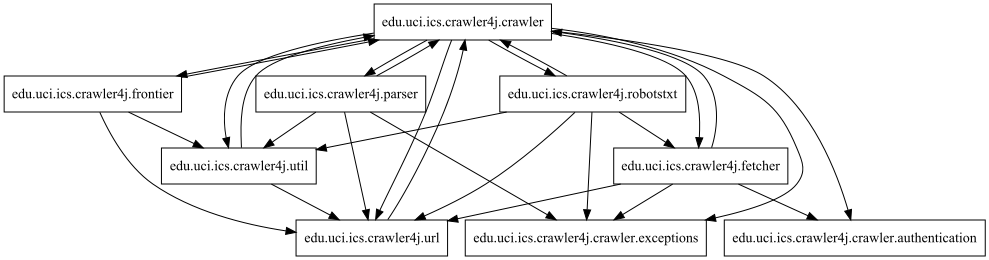
\includegraphics[scale=0.5]{img/crawler_packages_orig}
    \caption{\textit{crawler4j} sistemos struktūra}
    \label{fig:crawler_packages_orig}
\end{figure}

Atlikus sistemos kokybės matų analizę galima pamatyti sistemai būdingas problemas (pavyzdys~\ref{table:crawler},~\ref{table:crawlers}).
\begin{center}
    \begin{tabular}{|c|c|c|c|c|c|c|c|}
        \hline
        Paketo vardas & \textit{N} & \textit{A} & \textit{E} & \textit{S} & \textit{A} & \textit{D} & \textit{C} \\ [0.5ex]
        \hline\hline
        edu.uci.ics.crawler4j.crawler.authentication & 4 & 2 & 0 & 0.0 & 0.25 & 0.75 & 0\\
        \hline
        edu.uci.ics.crawler4j.url & 4 & 6 & 1 & 0.143 & 0.0 & 0.857 & 1 \\
        \hline
        edu.uci.ics.crawler4j.crawler.exceptions & 3 & 4 & 0 & 0.0 & 0.0 & 1.0 & 0\\
        \hline
        edu.uci.ics.crawler4j.crawler & 5 & 6 & 8 & 0.571 & 0.2 & 0.229 & 5 \\
        \hline
        edu.uci.ics.crawler4j.robotstxt & 6 & 1 & 5 & 0.833 & 0.0 & 0.167 & 1 \\
        \hline
        edu.uci.ics.crawler4j.frontier & 6 & 1 & 3 & 0.75 & 0.0 & 0.25 & 1 \\
        \hline
        edu.uci.ics.crawler4j.fetcher & 6 & 2 & 4 & 0.667 & 0.0 & 0.333 & 1 \\
        \hline
        edu.uci.ics.crawler4j.util & 3 & 4 & 2 & 0.333 & 0.0 & 0.667 & 0 \\
        \hline
        edu.uci.ics.crawler4j.parser & 12 & 1 & 4 & 0.8 & 0.167 & 0.033 & 1 \\
        \hline
        \label{table:crawler}
    \end{tabular}
    \begin{tabular}{|c|c|c|c|c|c|c|}
        \hline
        $\bar{N}$ & $\bar{Af}$ & $\bar{Ef}$ & $\bar{S}$ & $\bar{A}$ & $\bar{D}$ & $\Sigma C$  \\ [0.5ex]
        \hline\hline
        5 & 3 & 3 & 0.455 & 0.069 & 0.476 & 5\\
        \hline
    \label{table:crawlers}
    \end{tabular}
\end{center}
\textbf{Matų lentelės paaiškinimas}:
\begin{itemize}
    \item \textit{N} - matas žymintis klasių skaičių pakete.
    \item \textit{Af} - aferentinės jungtys. Nurodo, kiek kitų paketų priklauso nuo pasirinkto paketo.
    \item \textit{Ef} - eferentinės jungtys. Nurodo, nuo kiek kitų paketų priklauso pasirinktas paketas.
    \item \textit{S} - stabilumas. Rodo paketo atsparumą pokyčiams, reikšmės rėžiai - nuo nulio iki vieno, nulis visiškai stabilus paketas, o vienetas - visiškai nestabilus.
    \item \textit{A} - nurodo paketo abstraktumą, reikšmės rėžiai - nuo nulio iki vieno, nulis reiškia, kad paketas neturi abstrakčių klasių, o vienetas nurodo, kad pakete yra tik abstrakčios klasės.
    \item \textit{D} - Atstumas nuo pagrindinės sekos arba atstumas nuo sąryšio tarp stabilumo ir abstrakcijos, reikšmės rėžiai - nuo nulio iki vieno, nulis reiškia paketą, sutampantį su pagrindine seka,vienas - paketą, maksimaliai nutolusį nuo pagrindinės sekos, siekiama reikšmė - 0.
    \item \textit{C} - ciklinių priklausomybių matas, rodo ciklines priklausomybės, siekiama reikšmė - 0.
\end{itemize}
Kaip skaičiuojami matai aprašyta \hyperref[sec:matai]{paketų kokybės matų} skyriuje.

Iš bendros sistemos analizės bei matų lentelės rezultatų matomos kelios sistemos problemos -
\begin{itemize}
    \item \textbf{Problema numeris 1} - atlikus bendrą sistemos kodo analizę matoma,
    kad sistemos paketuose yra daug sąsajų su skirtingais jų įgyvendinimais, todėl yra sunku
    rasti visus specifinės sąsajos įgyvendinimus.
    \item \textbf{Problema numeris 2} - paketo \textit{edu.uci.ics.crawler4j.parser} viduje yra 12 klasių, todėl sunku suprasti, už kokius funkcionalumus jis atsakingas
    ir kada jį reikėtų nagrinėti bei keisti.
    \item \textbf{Problema numeris 3} - Sistema turi daug ciklinių prilausomynbių, kur du arba daugiau paketų priklauso vienas nuo kito.
    Tai matoma sistemos paketų diagramoje\ref{fig:crawler_packages_orig}, ciklinėse priklausomybėse dalyvauja 10 paketų ir kartu jie sudaro 5 ciklinių priklausomybių sekas,
    kurios turėtų būti pašalintos.
\end{itemize}

Sistemos paketas \textit{edu.uci.ics.crawler4j.parse}, turi sąsają \textit{ParseData} bei 4 skirtingus jos įgyvendinimus - \textit{CssParseData, TextParseData, HtmlParseData, BinaryParseData},
šios klasės pakete dalinasi vieta dar su 9 klasėmis, todėl yra nepatogu rasti ieškomą įgyvendinimą (pavyzdys~\ref{fig:parse}).
\begin{figure}[H]
    \snugshade
    \dirtree{%
        .1 {/parser} .
        .2 {AllTagMapper}.
        .2 {ParseData}.
        .3 {TextParseData}.
        .3 {HtmlParseData}.
        .2 {CssParseData}.
        .2 {BinaryParseData}.
        .2 {ExtractedUrlAnchorPair}.
        .2 {HtmlParser}.
        .2 {HtmlContentHandler}.
        .2 {TikaHtmlParser}.
        .2 {Parser}.
    }
    \endsnugshade
    \caption{\textit{parser} paketo struktūra}
    \label{fig:parse}
\end{figure}
Šiam paketui sutvarkyti taikomas \textit{įgyvendinimų atskyrimo} šablonas - sąsaja iškeliama į atskirą paketą \textit{parse}, jos įgyvendinimai perkeliami į minėto
paketo subpaketus.
Šie pertvarkymai pakeičia \textit{parser} paketo struktūrą (pavyzdys~\ref{fig:parser}).
\begin{figure}[H]
    \snugshade
    \dirtree{%
        .1 {/parser} .
        .2 {parse}.
        .3 {ParseData // Sąsaja}.
        .3 {text}.
        .4 {TextParseData // Pirmas sąsajos įgyvendinimas}.
        .3 {html }.
        .4 {HtmlParseData // Antras sąsajos įgyvendinimas}.
        .3 {css }.
        .4 {CssParseData // Trečias sąsajos įgyvendinimas}.
        .3 {binary}.
        .4 {BinaryParseData // Ketvirtas sąsajos įgyvendinimas}.
        .2 {AllTagMapper}.
        .2 {ExtractedUrlAnchorPair}.
        .2 {HtmlParser}.
        .2 {HtmlContentHandler}.
        .2 {NotAllowedContentException}.
        .2 {TikaHtmlParser}.
        .2 {Parser}.
    }
    \endsnugshade
    \caption{\textit{parser} paketo struktūra po pirmojo pertvarkymo}
    \label{fig:parser}
\end{figure}
Dėl atskirtos sąsajos ir jos įgyvendinimų tampa daug paprasčiau ją rasti bei suprasti sistemoje egzistuojančius jos įgyvendinimus.
Tokia struktūra išsprendžia sistemos \textbf{problemą numeris 1}.
Šis pertvarkymas taip pat dalinai sumažino \textbf{problemą numeris 2}, sumažinant klasių skaičių pakete į 7.
Palyginus pertvarkytos ir buvusios sitemos matus matome, kad sistema tapo aiškesnė, sumažėjo vidutinis klasių skaičius paketuose, nežymiai sumažėjo
vidutinis stabilumas, bet pakilo abstrakcijos lygis, todėl atstumas nuo pagrindinės sekos sumažėjo (pavyzdys~\ref{table:parser},~\ref{table:parsers}).
\begin{center}
    \begin{tabular}{|c|c|c|c|c|c|c|c|}
        \hline
        \textit{crawler4j.parser} & \textit{N} & \textit{A} & \textit{E} & \textit{S} & \textit{A} & \textit{D} & \textit{C} \\ [0.5ex]
        \hline\hline
        Prieš & 12 & 1 & 4 & 0.8 & 0.167 & 0.033 & 1 \\
        \hline
        Po & \cellcolor{green!25} 7 (-5) & 1 & 9 & \cellcolor{red!25} 0.9 + (0.1) & \cellcolor{red!25} 0.143 (-0.024) & \cellcolor{red!25} 0.043 (+0.01) & 1 \\
        \hline
        \label{table:parser}
    \end{tabular}
    \begin{tabular}{|c|c|c|c|c|c|c|c|}
        \hline
        Vidurkiai & $\bar{N}$ & $\bar{Af}$ & $\bar{Ef}$ & $\bar{S}$ & $\bar{A}$ & $\bar{D}$ & $\Sigma C$ \\ [0.5ex]
        \hline\hline
        Prieš & 5 & 3 & 3 & 0.455 & 0.069 & 0.476 & 5\\
        \hline
        Po & \cellcolor{green!25} 4 (-1) & 3 & 3 & \cellcolor{red!25} 0.488 (+0.033) & \cellcolor{green!25} 0.114 (+0.045) & \cellcolor{green!25} 0.425 (-0.051) & 5 \\
        \hline
        \label{table:parsers}
    \end{tabular}
\end{center}
Matų pokyčio didėjimas nebūtinai susijęs su sistemos kokybės gerėjimu, todėl teigiamas pokytis paženklintas žaliai, o neigiamas - raudonai.
Norint išspręsti \textbf{problemą numeris 3} - ciklines priklausomybes, reikia identifikuoti klases, kurių priklausomybės
sudaro ciklus ir iškelti jas į atskirus paketus.

Kuriant naujus paketus vadovaujamasi \textit{skirstymo pagal smulkų funkcionalumą} šablonu, užtikrinant, kad kiekvienas
paketas teikia vieną, aiškiai apibrėžtą funkciją, kuri yra pasiekiama per pakete aprašytą sąsają.
Paketo vidus yra paslėptas su \textit{Java} kalbos pasiekiamumo modifikatoriais - konkrečių klasių negalima inicializuoti už paketo ribų,
nes jų konstruktoriai privatūs (pavyzdys~\ref{fig:sasaja}).

\begin{figure}[H]
    \begin{lstlisting}[language=Python]
public interface HtmlParser {

    HtmlParseData parse(ParsedPage page, String contextURL) throws ParseException;

    // Grazinamas sasajos igyvendinimas
    static HtmlParser newHtmlParser(CrawlConfig config, TLDList tldList) throws InstantiationException, IllegalAccessException {
        return new TikaHtmlParser(config, tldList);
    }
}

// Sasajos igyvendinimas. Nera viesas, pasiekiamas tik paketo viduje, nes klase ir konstruktorius nenaudoja public raktazodziu
class TikaHtmlParser implements HtmlParser {
   ...
    TikaHtmlParser(CrawlConfig config, TLDList tldList) throws InstantiationException, IllegalAccessException {
     ...
    }
    \end{lstlisting}
    \caption{\textit{skirstymo pagal teikiamą funkcionalumą} šablono sąsaja}
    \label{fig:sasaja}
\end{figure}
Peržiūrėjus paketus su ciklinėmis priklausomybėmis, iš jų buvo išskirti šie nauji funkcionalumai, kuriems
buvo sukurti atskiri paketai (pavyzdys~\ref{fig:crawlerj},~\ref{fig:crawlerjs}).
\begin{itemize}
    \item Iš \textit{parser} paketo iškeltas funkcionalumas \textit{html} turiniui apdoroti, patalpintas į \textit{parser/html} paketą.
    Po šio pertvarkymo \textit{parser} paketas pasidaro mažesnis ir turi vieną funkcionalumą - priimti puslapį ir deleguoti jį apdorojimui kitai klasei pagal puslapio tipą.
    \item Iš \textit{robotstxt} paketo funkcionalumas patikrinti, ar sistema autorizuota apdoroti pasirinktą puslapį, iškeltas į \textit{robotstxt/permissions} paketą.
    \item Iš \textit{crawler}, bei \textit{parser} paketų funkcionalumas, aprašantis internetinio puslapio elementus, iškeltas į \textit{web} paketą.
    \item Iš \textit{crawler} paketo funkcionalumas, nustatantis įrankio konfigūraciją, iškeltas į \textit{config} paketą.
    \item Iš \textit{url} paketo funkcionalumas, gaunantis internetinių domenų pavadinimus, iškeltas į \textit{tld} paketą.
\end{itemize}

\begin{figure}[H]
    \snugshade
    \dirtree{%
        .1 {/} .
        .2 {crawler4j}.
        .3 {crawler}.
        .4 {authentication}.
        .4 {exceptions}.
        .3 {fetcher}.
        .3 {frontier}.
        .3 {parser}.
        .4 {parse}.
        .5 {binary}.
        .5 {css}.
        .5 {factory}.
        .5 {html}.
        .5 {text}.
        .3 {robotstxt}.
        .3 {url}.
        .3 {util}.
    }
    \endsnugshade
    \caption{\textit{crawler4j} paketų medis prieš iškeliant minėtus funkcionalumus}
    \label{fig:crawlerj}
\end{figure}

\begin{figure}[H]
    \snugshade
    \dirtree{%
        .1 {/} .
        .2 {crawler4j}.
        .3 {config}.
        .3 {crawler}.
        .4 {authentication}.
        .3 {fetcher}.
        .3 {frontier}.
        .3 {parser}.
        .4 {html}.
        .4 {parse}.
        .5 {binary}.
        .5 {css}.
        .5 {html}.
        .5 {text}.
        .3 {robotstxt}.
        .4 {permissions}.
        .3 {tld}.
        .3 {util}.
        .3 {web}.
    }
    \endsnugshade
    \caption{\textit{crawler4j} paketų medis iškėlus minėtus funkcionalumus}
    \label{fig:crawlerjs}
\end{figure}

Atlikus šiuos funkcionalumų suskaidymus į atskirus paketus buvo panaikintos žiedinės priklausomybės.
Naujoje paketų diagramoje galime matyti, jog dabar sistema turi daugiau paketų, tačiau jų priklausomybių kryptys daug aiškesnės (pavyzdys~\ref{img:crawler_packages_v2}).
\subsection{\textit{Crawler} sistema}
\begin{figure}[H]
    \centering
    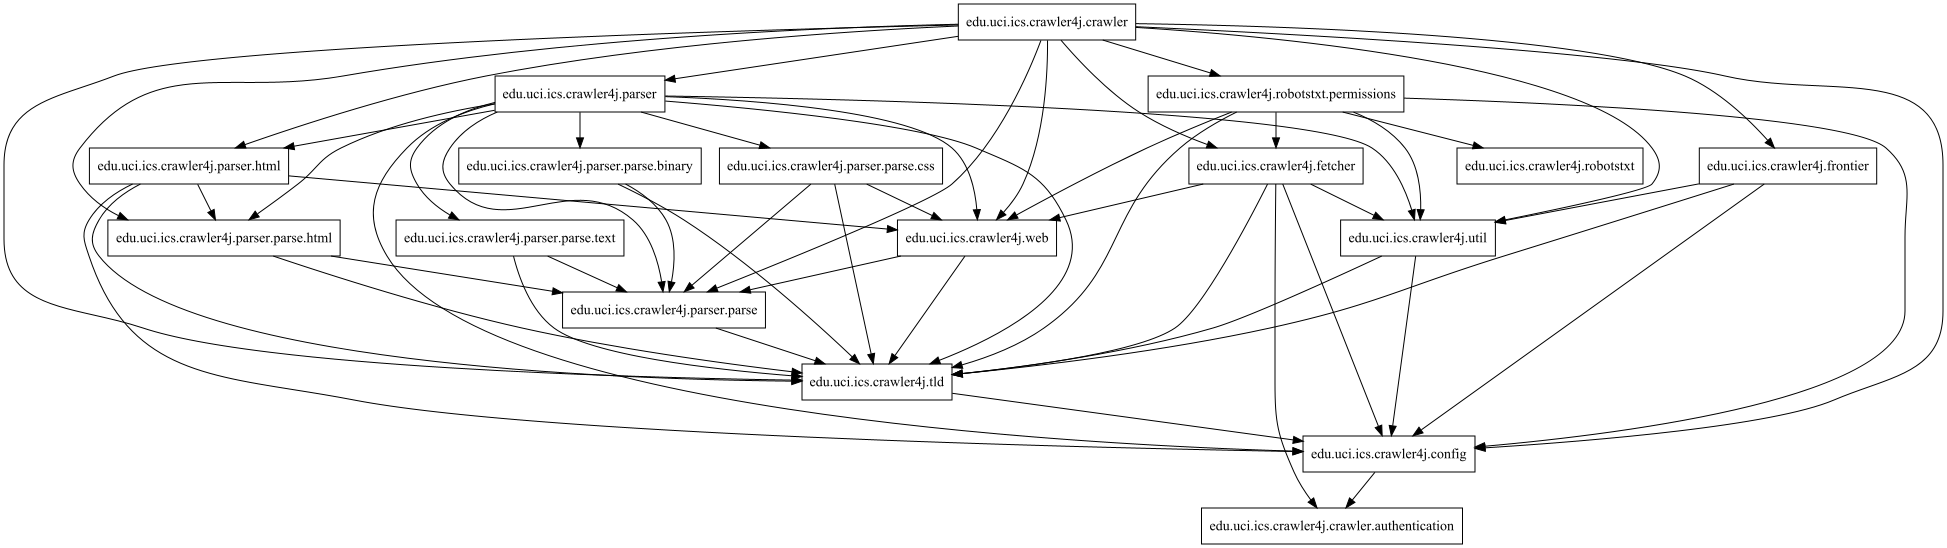
\includegraphics[scale=0.2]{img/crawler_packages_v2}
    \caption{\textit{crawler4j} sistemos struktūra po antro pertvarkymo}
    \label{img:crawler_packages_v2}
\end{figure}

Atlikus matų analizę pertvarkytai sistemai yra matoma, kad sistemos kokybė pagerėjo,
sumažėjo vidutinis klasių skaičius pakete, ciklinių priklausomybių rodiklis tapo lygus nuliui,
padidėjo vidutinis abstrakcijos lygis (pavyzdys~\ref{table:abstr},~\ref{table:abstrs}).
\begin{center}
    \begin{tabular}{|c|c|c|c|c|c|c|c|}
        \hline
        Paketo vardas & \textit{N} & \textit{Af} & \textit{Ef} & \textit{S} & \textit{A} & \textit{D} & \textit{C} \\ [0.5ex]
        \hline\hline
        edu.uci.ics.crawler4j.parser.parse.binary & 1 & 1 & 2 & 0.667 & 0.0 & 0.333 & 0 \\
        \hline
        edu.uci.ics.crawler4j.crawler & 4 & 0 & 11 & 1.0 & 0.25 & 0.25 & 0 \\
        \hline
        edu.uci.ics.crawler4j.tld & 3 & 13 & 1 & 0.071 & 0.333 & 0.596 & 0 \\
        \hline
        edu.uci.ics.crawler4j.parser.html & 6 & 2 & 4 & 0.667 & 0.167 & 0.166 & 0 \\
        \hline
        edu.uci.ics.crawler4j.robotstxt.permissions & 2 & 1 & 6 & 0.857 & 0.5 & 0.357 & 0 \\
        \hline
        edu.uci.ics.crawler4j.config & 1 & 8 & 1 & 0.111 & 0.0 & 0.889 & 0 \\
        \hline
        edu.uci.ics.crawler4j.frontier & 6 & 1 & 3 & 0.75 & 0.0 & 0.25 & 0 \\
        \hline
        edu.uci.ics.crawler4j.parser & 2 & 1 & 10 & 0.909 & 0.0 & 0.091 & 0\\
        \hline
        edu.uci.ics.crawler4j.crawler.authentication & 4 & 2 & 0 & 0.0 & 0.25 & 0.75 & 0 \\
        \hline
        edu.uci.ics.crawler4j.parser.parse.css & 1 & 1 & 3 & 0.75 & 0.0 & 0.25 & 0 \\
        \hline
        edu.uci.ics.crawler4j.robotstxt & 5 & 1 & 0 & 0.0 & 0.0 & 1.0 & 0 \\
        \hline
        edu.uci.ics.crawler4j.parser.parse.html & 1 & 3 & 2 & 0.4 & 0.0 & 0.6 & 0 \\
        \hline
        edu.uci.ics.crawler4j.parser.parse & 1 & 7 & 1 & 0.125 & 1.0 & 0.125 & 0\\
        \hline
        edu.uci.ics.crawler4j.fetcher & 6 & 2 & 5 & 0.714 & 0.0 & 0.286 & 0 \\
        \hline
        edu.uci.ics.crawler4j.util & 4 & 5 & 2 & 0.286 & 0.0 & 0.714 & 0 \\
        \hline
        edu.uci.ics.crawler4j.web & 5 & 6 & 2 & 0.25 & 0.4 & 0.35 & 0 \\
        \hline
        edu.uci.ics.crawler4j.parser.parse.text & 1 & 1 & 2 & 0.667 & 0.0 & 0.333 & 0 \\
        \hline
        \label{table:abstr}
    \end{tabular}
    \begin{tabular}{|c|c|c|c|c|c|c|c|}
        \hline
        Vidurkiai & $\bar{N}$ & $\bar{Af}$ & $\bar{Ef}$ & $\bar{S}$ & $\bar{A}$ & $\bar{D}$ & $\Sigma C$ \\ [0.5ex]
        \hline\hline
        Prieš & 5 & 3 & 3 & 0.455 & 0.069 & 0.476 & 5\\
        \hline
        Po & \cellcolor{green!25} 3 (-2) & 3 & 3 & \cellcolor{green!24} 0.452 (-0.03) & \cellcolor{green!25} 0.183 (+0.114) & \cellcolor{green!25} 0.471 (-0.005) & \cellcolor{green!25} 0 (-5)\\
        \hline
    \label{table:abstrs}
    \end{tabular}
\end{center}
Iš gautų rezultatų galime teigti, jog po pertvarkymo šablonai \textit{skirstymas pagal smulkų funkcionalumą} ir \textit{įgyvendinimų atskyrimas}, išsprendė visas 3 sistemoje matytas problemas,
padarė sistemą lengviau suprantama, panaikino ciklines priklausomybes ir turėjo teigiamą įtaką matams, nurodantiems
sistemos įgyvendinimo kokybę.


\subsection{\textit{azure-sdk-for-java} sistema}
\textbf{azure-sdk-for-java\footnote{\url{https://github.com/Azure/azure-sdk-for-java/tree/main/sdk/storage/azure-storage-blob-cryptography}}} yra atviro kodo
biblioteka, parašyta \textit{Java} programavimo kalba, leidžianti programiškai bendrauti su \textit{Microsoft Azure} debesų kompiuterijos platforma.
Tai programinės įrangos įrankis, skirtas naudoti kitose sistemose, supaprastinant programinį kodą.
Ši biblioteka yra labai didelė ir šio pertvarkymo metu yra dirbama tik su posisteme \textit{azure-storage-blob-cryptograph}, kuri atsakinga už duomenų kriptografiją
komunikacijos su \textit{Azure Blog} nestruktūrizuota failų saugykla metu.

Prieš visus pakeitimus \textit{azure-storage-blob-cryptograph} sistema turi vieną paketą \textit{com.azure.storage.blob.specialized.cryptography}, kuriame guli visos jos klasės.

Sistemos kokybės matai nėra naudingi dirbant su vienu paketu, nes trūksta konteksto suprasti, kaip paketas yra naudojamas.
Tačiau iš bendrinės sistemos analizės galima pamatyti pagrindines sistemos problemas - viename pakete yra 21 skirtinga klasė, tiek sąsajos, tiek konkrečios klasės.
Taip pat sistemoje yra kelios skirtingos tos pačios esybės versijos - \textit{DecryptorV1} ir \textit{DecryptorV2}, \textit{EncryptorV1} ir \textit{EncryptorV2}, todėl sunku
suprasti, su kokia esybės versija yra susijusios kitos klasės bei yra kodo pasikartojimo.
Ši sistema būtų aiškesnė ir greičiau perprantama, jei būtų išskirti mažesni funcionalumai ir kodas būtų išskaidytas į smulkesnius paketus, taip pat atskiriant juos
pagal esybių versijas.
Norint atlikti esybių versijavimą naudojamas \textit{skirtingų versijų grupavimo į paketus} šablonas, pagal jį kiekvienai esybės versijai sukuriamas atskiras paketas,
taip pat bendras, pasikartojantis kodas iškeliamas į abstrakčią klasę, kuri yra pakete vienu lygiu auksčiau nei versijų paketai (pavyzdys~\ref{fig:rep}).
\begin{figure}[H]
    \snugshade
        \dirtree{%
            .1 {/cryptography} .
            .2 {decryptor} .
            .3 {Decryptor // Abstrakti klasė su bendru esybės kodu} .
            .3 {v1} .
            .4 {DecryptorV1 // Pirma esybės versija} .
            .3 {v2} .
            .4 {DecryptorV2 // Antra esybės versija} .
            .2 {encryptor} .
            .3 {Encryptor // Abstrakti klasė su bendru esybės kodu} .
            .3 {agent // Papildomas, su esybe susijęs kodas, naudojamas abiejų esybių} .
            .3 {v1} .
            .4 {EncryptorV1 // Pirma esybės versija} .
            .3 {v2} .
            .4 {EncryptorV2 // Antra esybės versija} .
        }
    \endsnugshade
    \caption{\textit{azure-storage-blob-cryptograph} paketų medis su paketais, skirtais esybių versijų valdymui}
    \label{fig:rep}
\end{figure}
Šis pertvarkymas pagal \textit{skirtingų versijų grupavimo į paketus} šabloną, atskiria esybės versijas ir pristato kelis paketus, apibrėžiančius aiškesnius funkcionalumus.
Atsiradus daugiau paketų bei jų sąsajų, galima paskaičiuoti paketų kokybės matus:
\begin{center}
    \begin{tabular}{|c|c|c|c|c|c|c|c|}
        \hline
        Paketo vardas & \textit{N} & \textit{Af} & \textit{Ef} & \textit{S} & \textit{A} & \textit{D} & \textit{C} \\ [0.5ex]
        \hline\hline
        specialized.cryptography & 13 & 7 & 5 & 0.417 & 0.0 & 0.583 & 5 \\
        \hline
        specialized.cryptography.encryptor.v2 & 1 & 1 & 3 & 0.75 & 0.0 & 0.25 & 0 \\
        \hline
        specialized.cryptography.encryptor.v1 & 1 & 0 & 3 & 1.0 & 0.0 & 0.0 & 1 \\
        \hline
        specialized.cryptography.encryptor & 1 & 4 & 2 & 0.333 & 1.0 & 0.333 & 2 \\
        \hline
        specialized.cryptography.decryptor.v2 & 1 & 1 & 2 & 0.667 & 0.0 & 0.333 & 1 \\
        \hline
        specialized.cryptography.decryptor.v1 & 1 & 1 & 2 & 0.667 & 0.0 & 0.333 & 1\\
        \hline
        specialized.cryptography.encryptor.agent & 2 & 3 & 2 & 0.4 & 0.0 & 0.6 & 1\\
        \hline
        specialized.cryptography.decryptor & 2 & 3 & 1 & 0.25 & 0.5 & 0.25 & 1 \\
        \hline
    \label{table:matai}
    \end{tabular}
    \begin{tabular}{|c|c|c|c|c|c|c|}
        \hline
        $\bar{N}$ & $\bar{Ag}$ & $\bar{Eg}$ & $\bar{S}$ & $\bar{A}$ & $\bar{D}$ & $\Sigma C$ \\ [0.5ex]
        \hline\hline
        3 & 3 & 3 & 0.561 & 0.188 & \cellcolor{green!25} 0.335 & \cellcolor{red!25} 6 \\
        \hline
    \label{table:matais}
    \end{tabular}
\end{center}
Apskaičiuoti matai (pavyzdys~\ref{table:matai},~\ref{table:matais})rodo nedidelį nuokrypį nuo pagrindinės sekos, todėl galima teigti, kad sistemos abstraktumas bei stabilumas
yra subalansuoti, tačiau šis skirstymas turėjo ir neigiamų padarinių - sukelė 6 ciklines priklausomybes.
Šiais priklausomybes galima matyti sistemos paketų diagramoje (pavyzdys~\ref{fig:azure_packages_v1}).
\begin{figure}[H]
    \centering
    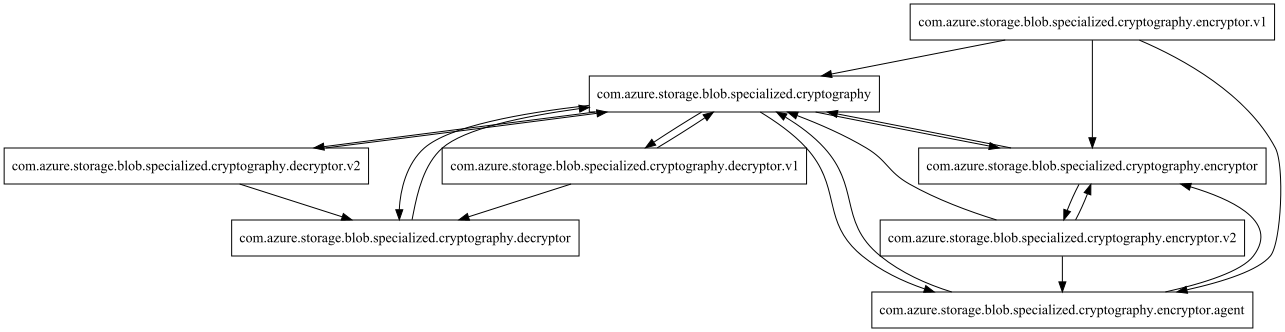
\includegraphics[scale=0.3]{img/azure_packages_v1}
    \caption{\textit{azure-storage-blob-cryptograph} sistemos struktūra po pirmojo pertvarkymo}
    \label{fig:azure_packages_v1}
\end{figure}
Norint panaikinti ciklines priklausomybes, reikia panaudoti šabloną \textit{skirstymas pagal smulkų funkcionalumą} ir, išskaidant pagrindinį paketą
į dar smulkesnius vienetus - yra sukuriamas \textit{encription.data} paketas, atsakingas už užkoduotų duomenų vaizdavimą, taip pat
aprašomas paketas \textit{blob} skirtas \textit{blob} esybių, reprezentuojančių saugyklos duomenų formatą, kriptografijai.
Taip pat vadovaujantis \textit{atskiro pagalbinių klasių paketo} šablonu, visos pagalbinės klasės, neturinčios priklausomybių į kitus paketus ir
padedančios vykdyti kertinius funcionalumus yra iškeliamos į \textit{util} paketą.
Minėtame pakete atsiranda tokios klasės:
\begin{itemize}
    \item \textit{CryptographyConstants} - klasė, saugojanti bendras, su kriptografija susijusias konstantas, kurios naudojamos skirtingose sistemos vietose.
    \item \textit{EncryptionVersion} - aprašo kriptografijos versijas ir jų naudojamus protokolus
    \item \textit{WrappedKeyJson} - palengvina darbą su serializuojant ir deserializuojant kriptografijos raktus į \textit{json} formatą.
\end{itemize}

Pritaikius visus šiuos šablonus, gaunama sistemos struktūra turinti nedidelius, aiškesniais funkcionalumais apibrėžtus paketus,
taip pat pašalinamos ciklinės priklausomybės (pavyzdys~\ref{fig:azure_packages_v2}).
\begin{figure}[H]
    \centering
    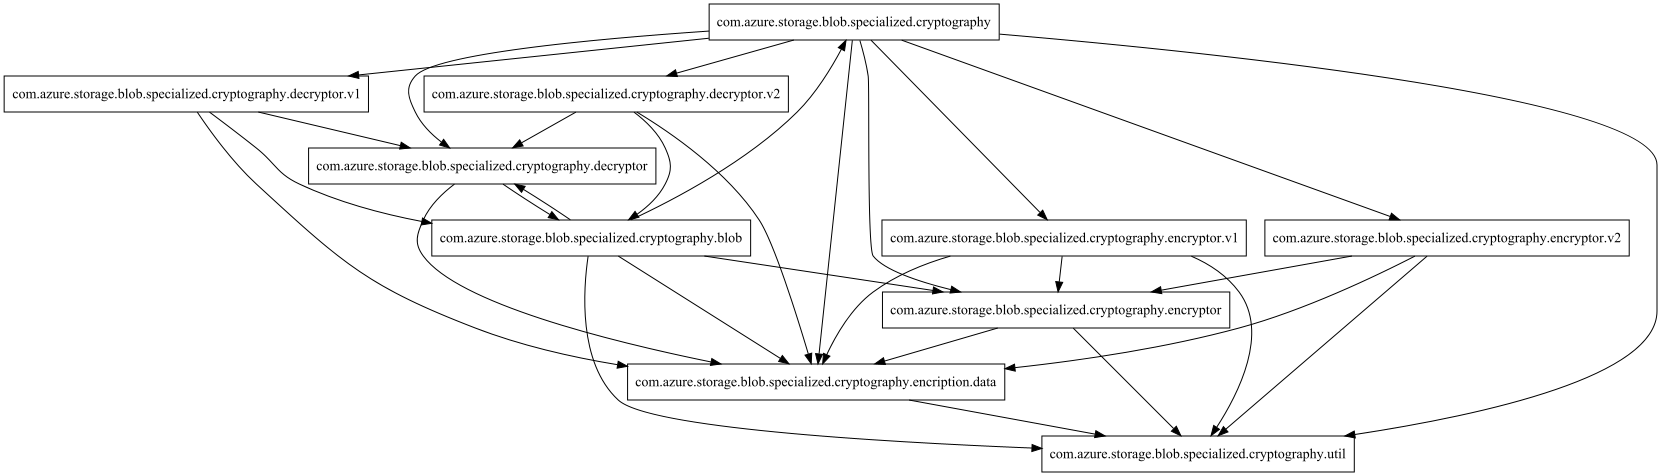
\includegraphics[scale=0.3]{img/azure_packages_v2}
    \caption{Galutinė \textit{azure-storage-blob-cryptograph} sistemos struktūra}
    \label{fig:azure_packages_v2}
\end{figure}

Pakartotinai įvertinus matus matoma, kad nuokrypis nuo pagrindinės sekos šiek tiek padidėjo, tačiau
vis dar yra gan mažas, ciklinės priklausomybės išnyko, todėl galime teigti, kad \textit{skirstymo pagal smulkų funkcionalumą},
\textit{atskiro pagalbinių klasių paketo} ir \textit{skirtingų versijų grupavimo į paketus} šablonai prisidėjo prie bendro
sistemos suprantamumo, įvedė aiškesnę jos struktūrą, išlaikant objektyviai gerus sistemos kokybės matus (pavyzdys~\ref{table:vert},~\ref{table:verts}).
\begin{center}
    \begin{tabular}{|c|c|c|c|c|c|c|c|}
        \hline
        Paketo vardas & \textit{N} & \textit{Af} & \textit{Ef} & \textit{S} & \textit{A} & \textit{D} & \textit{C} \\ [0.5ex]
        \hline\hline
        specialized.cryptography & 3 & 1 & 8 & 0.889 & 0.0 & 0.111 & 0 \\
        \hline
        specialized.cryptography.blob & 6 & 3 & 5 & 0.625 & 0.0 & 0.375 & 0 \\
        \hline
        specialized.cryptography.encription.data & 4 & 8 & 1 & 0.111 & 0.0 & 0.889 & 0 \\
        \hline
        specialized.cryptography.encryptor.v2 & 1 & 1 & 3 & 0.75 & 0.0 & 0.25 & 0 \\
        \hline
        specialized.cryptography.encryptor.v1 & 1 & 1 & 3 & 0.75 & 0.0 & 0.25 & 0 \\
        \hline
        specialized.cryptography.encryptor & 1 & 4 & 2 & 0.333 & 1.0 & 0.333 & 0 \\
        \hline
        specialized.cryptography.decryptor.v2 & 1 & 1 & 3 & 0.75 & 0.0 & 0.25 & 0 \\
        \hline
        specialized.cryptography.decryptor.v1 & 1 & 1 & 3 & 0.75 & 0.0 & 0.25 & 0 \\
        \hline
        specialized.cryptography.decryptor & 2 & 4 & 2 & 0.333 & 0.5 & 0.167 & 0 \\
        \hline
        specialized.cryptography.util & 3 & 6 & 0 & 0.0 & 0.0 & 1.0 & 0 \\
        \hline
    \label{table:vert}
    \end{tabular}
    \begin{tabular}{|c|c|c|c|c|c|c|c|}
        \hline
        Vidurkiai & $\bar{N}$ & $\bar{A}$ & $\bar{E}$ & $\bar{S}$ & $\bar{A}$ & $\bar{D}$ & $\Sigma C$ \\ [0.5ex]
        \hline\hline
        Pirmas pertvarkymas & 3 & 3 & 3 & 0.561 & 0.188 & 0.335 & 6 \\
        Galutinis variantas & \cellcolor{green!25} 2 (-1) & 3 & 3 & \cellcolor{green!25} 0.529 (-0.032) & \cellcolor{red!25} 0.15 (-0.03) & \cellcolor{red!25} 0.388 (+0.053) &  \cellcolor{green!25} 0 (-5) \\
        \hline
        \label{table:verts}
    \end{tabular}
\end{center}
